
%----------------------------------------------------------------------------
\chapter{Overview of the approach}
%----------------------------------------------------------------------------

%%
%% Futásidejű dolgok és kódgenerálás is!
%%

In this chapter, I present the approach to monitoring of cyber-physical systems, that the developed framework uses. It is depicted on figure~\ref{fig:approach}. Mainly we can divide the framework usage or domain to two main section: design time and runtime. 

\begin{figure}[h]
	\begin{center}
		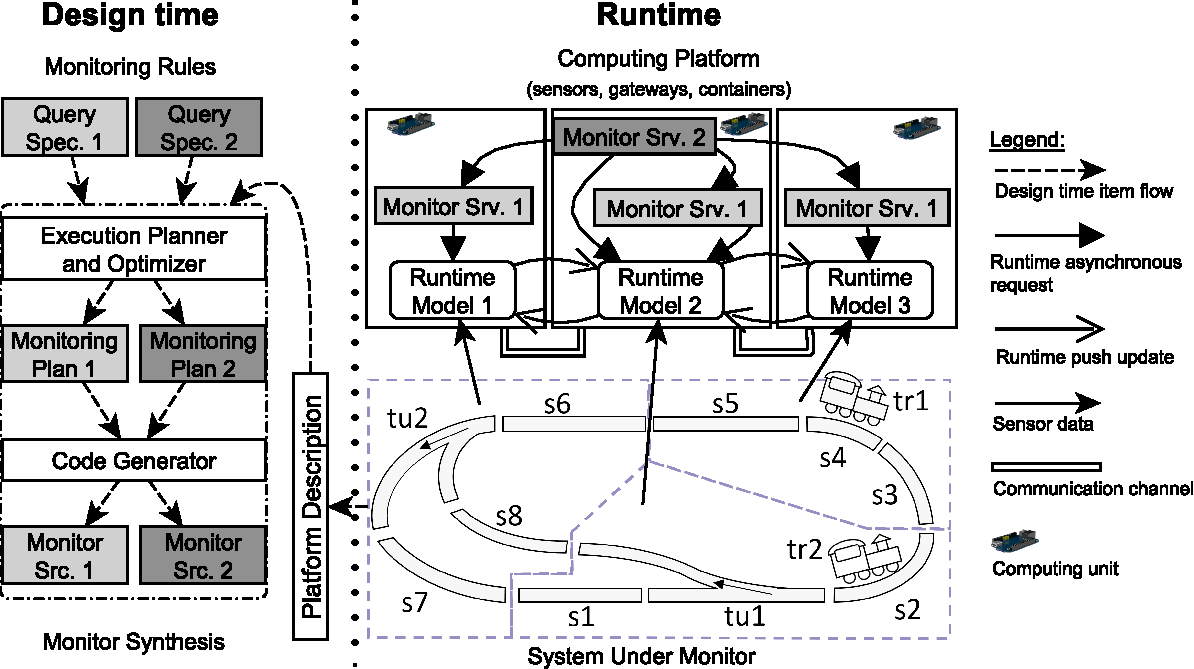
\includegraphics[width=\textwidth]{figures/fase-overview-crop.pdf}
		\caption{Approach for cyber-physical systems monitoring used by the presented framework }
		\label{fig:approach}
	\end{center}
\end{figure}


At first, we design the models based on the structure of the target system. The metamodel of the living model defines the types of the graph elements, the possible edges between instances of given types, and attributes of instances of a given type. For this we use EMF Ecore modeling. This model is similar to a UML class diagram unless it only describes structural features. We generate \cpp{} classes from these models, that can be used to build up and update the living model of the system.

Monitoring goals are defined as graph patterns. For graph pattern definition, the query language of \viatra{} is used (vql). From these patterns we create monitoring plans, ie.\ local search strategies. We use these plans to generate the source code of the monitoring components.

At runtime, we rely on the generated monitor code and the generated classes. By instancing the classes, we create the nodes of the living model, create the references/edges between them and give the values of the attributes of the objects. With the physical world changing we update the objects to reflect the current state of the system. On this model, we run the monitoring code to find matches for the pattern in the model. If a pattern match occurs, we find the model elements that conform the pattern, thus we can locate the problems in the model, and through the model, in the physical world. 

